%%
%% INTUNE: Self-Improving LLM via Incremental Knowledge Distillation
%% ACM sigconf format
%%
\documentclass[sigconf]{acmart}
\makeatletter
\@ACM@balancefalse
\makeatother

\setcopyright{none}
\copyrightyear{2026}
\acmYear{2026}
\acmDOI{}
\acmConference[AIDM'26]{ACM International Conference on AI and Data Management}{2026}{}
\acmISBN{}

\usepackage{booktabs}
\usepackage{multirow}
\usepackage{amsmath}
\usepackage{graphicx}
\usepackage{xcolor}
\usepackage{tikz}
\usetikzlibrary{shapes.geometric, arrows.meta, positioning, fit, backgrounds}
\usepackage{pgfplots}
\pgfplotsset{compat=1.18}

\definecolor{darkblue}{RGB}{0,51,102}
\definecolor{lightblue}{RGB}{230,240,250}

\begin{document}
\raggedbottom

\title{INTUNE: Incremental Knowledge Distillation with Training Dynamics Analysis for Compact LLMs}

\author{Radhakrishna Bharuka}
\affiliation{\institution{}}
\email{radhebharuka29@gmail.com}

\author{Abhang Pawar}
\affiliation{\institution{}}
\email{abhangpawar03@gmail.com}

\author{Nilesh Dwivedi}
\affiliation{\institution{}}
\email{nileshdwivedi195@gmail.com}

\author{Rushikesh Masalkar}
\affiliation{\institution{}}
\email{rushikeshmasalkar00@gmail.com}

%% ===== ABSTRACT =====
\begin{abstract}
Large language models have achieved remarkable performance across diverse tasks, yet their deployment on resource-constrained devices remains challenging due to computational and memory requirements. Knowledge distillation offers a promising solution by transferring learned behaviors from a large teacher model to a compact student model. However, prior work lacks systematic methodologies for teacher selection and provides limited insight into training dynamics during the distillation process. We present INTUNE, a two-phase framework that addresses these gaps through (1) a bias-free teacher selection mechanism using seven model-agnostic evaluation metrics, and (2) an incremental training pipeline that enables fine-grained analysis of learning progression across ten checkpoints. Our experiments on 50,000 instruction-following samples demonstrate that a well-aligned 7B-parameter teacher (Alpaca) outperforms a larger 20B-parameter alternative (GPT-NeoX) by achieving 40\% lower hallucination rates despite having fewer parameters. While batch training achieves marginally higher final performance, incremental training provides critical interpretability benefits including learning curve visualization, diminishing returns detection at approximately 30K samples, and early identification of catastrophic forgetting. To address the computational bottleneck of repeated checkpoint evaluation across 50K samples, we additionally propose an event-driven pipeline architecture that automates training triggers and enables parallel evaluation, reducing manual intervention and enabling scalable workflows. INTUNE positions knowledge distillation as an analytical framework for understanding training behavior rather than solely optimizing final accuracy.
\end{abstract}

\begin{CCSXML}
<ccs2012>
<concept>
<concept_id>10010147.10010178.10010224.10010225</concept_id>
<concept_desc>Computing methodologies~Natural language processing</concept_desc>
<concept_significance>500</concept_significance>
</concept>
</ccs2012>
\end{CCSXML}
\ccsdesc[500]{Computing methodologies~Natural language processing}
\keywords{knowledge distillation, large language models, incremental learning, model compression}

\maketitle

%% ===== 1. INTRODUCTION =====
\section{Introduction}

The rapid advancement of large language models (LLMs) has transformed natural language processing, enabling unprecedented performance on tasks ranging from question answering to code generation. Models such as GPT-4, LLaMA, and Gemma have demonstrated emergent capabilities that scale with parameter count, yet this scaling comes at significant computational cost. Deploying billion-parameter models requires specialized hardware, substantial memory, and considerable energy consumption, limiting their accessibility for edge devices, mobile applications, and cost-sensitive deployments.

Knowledge distillation~\cite{hinton2015distilling} provides an elegant solution by training a compact student model to mimic the behavior of a larger teacher model. Rather than compressing model weights directly, distillation transfers learned representations through the teacher's output distributions, enabling students to achieve competitive performance with substantially fewer parameters. However, existing distillation approaches face two critical limitations: they typically assume that larger teachers produce better students without systematic validation, and they provide limited visibility into how learning progresses during training, making it difficult to identify optimal data budgets or detect training pathologies.

We introduce INTUNE (Incremental kNowledge disTillation Using iNcrEmental training), a framework designed to address both limitations. INTUNE operates in two phases: first, it systematically compares candidate teacher models using a suite of seven model-agnostic metrics that evaluate output quality without relying on LLM-as-judge approaches, which are known to exhibit position bias and self-preference~\cite{zheng2023judging}. Second, it trains the student incrementally across ten checkpoints, generating learning curves that reveal diminishing returns, catastrophic forgetting, and per-metric evolution. This incremental approach prioritizes interpretability over raw performance, providing actionable insights for practitioners optimizing training budgets or debugging model behavior.

Our contributions are as follows: (1) A systematic teacher selection framework demonstrating that Alpaca-7B achieves 47\% overall score with 40\% lower hallucination than GPT-NeoX-20B, challenging the assumption that larger teachers are always superior. (2) Comprehensive analysis of incremental versus batch training dynamics, showing that while batch training achieves marginally higher final scores (projected 0.6\% improvement), incremental training reveals performance plateaus around 30K samples where 90\% of gains occur at 60\% of compute cost. (3) An event-driven pipeline architecture that addresses the computational bottleneck of repeated checkpoint evaluation by automating training triggers and enabling parallel metric computation, making large-scale incremental distillation studies feasible.

%% ===== 2. RELATED WORK =====
\section{Related Work}

\paragraph{Knowledge Distillation.}
Hinton et al.~\cite{hinton2015distilling} introduced knowledge distillation by training students on soft probability distributions from teacher models, enabling knowledge transfer beyond hard labels. Subsequent work applied this paradigm to language models: DistilBERT~\cite{sanh2019distilbert} achieved 97\% of BERT's performance with 40\% fewer parameters through task-agnostic distillation; TinyBERT~\cite{jiao2020tinybert} introduced layer-wise attention transfer for deeper compression; MiniLM~\cite{wang2020minilm} proposed self-attention distillation achieving state-of-the-art efficiency. These approaches focus on architectural compression and performance preservation. INTUNE differs by prioritizing training interpretability: we analyze learning dynamics across incremental checkpoints rather than optimizing solely for final accuracy, revealing insights about data efficiency and catastrophic forgetting invisible to single-pass methods.

\paragraph{Teacher Model Selection.}
Most distillation research assumes a predefined teacher, typically the largest available model. West et al.~\cite{west2022symbolic} explored symbolic knowledge extraction from GPT-3, while Taori et al.~\cite{taori2023alpaca} demonstrated effective instruction-following through self-instruct on LLaMA. However, systematic comparison of teacher effectiveness remains understudied. Our work contributes a bias-free evaluation framework using seven heuristic metrics (structured correctness, task success, instruction following, coverage, faithfulness, hallucination, context grounding) that avoid LLM-as-judge approaches. We demonstrate empirically that smaller, well-aligned teachers can outperform larger alternatives when hallucination control is prioritized.

\paragraph{Incremental and Curriculum Learning.}
Curriculum learning~\cite{bengio2009curriculum} improves training by presenting examples in increasing difficulty order. Progressive Neural Networks~\cite{rusu2016progressive} address catastrophic forgetting through lateral connections between task-specific columns. Elastic Weight Consolidation~\cite{kirkpatrick2017overcoming} preserves important weights during sequential learning. INTUNE's incremental approach differs in studying data-scale progression (5K$\rightarrow$50K samples) rather than difficulty-based curricula, enabling analysis of when additional data yields diminishing returns and whether batch versus incremental training produces different convergence behaviors.

%% ===== 3. APPROACH =====
\section{Approach}

\subsection{System Architecture}

Figure~\ref{fig:architecture} presents the INTUNE system architecture comprising three integrated components: teacher selection, dual-path training comparison, and event-driven orchestration.

\begin{figure*}[t]
\centering
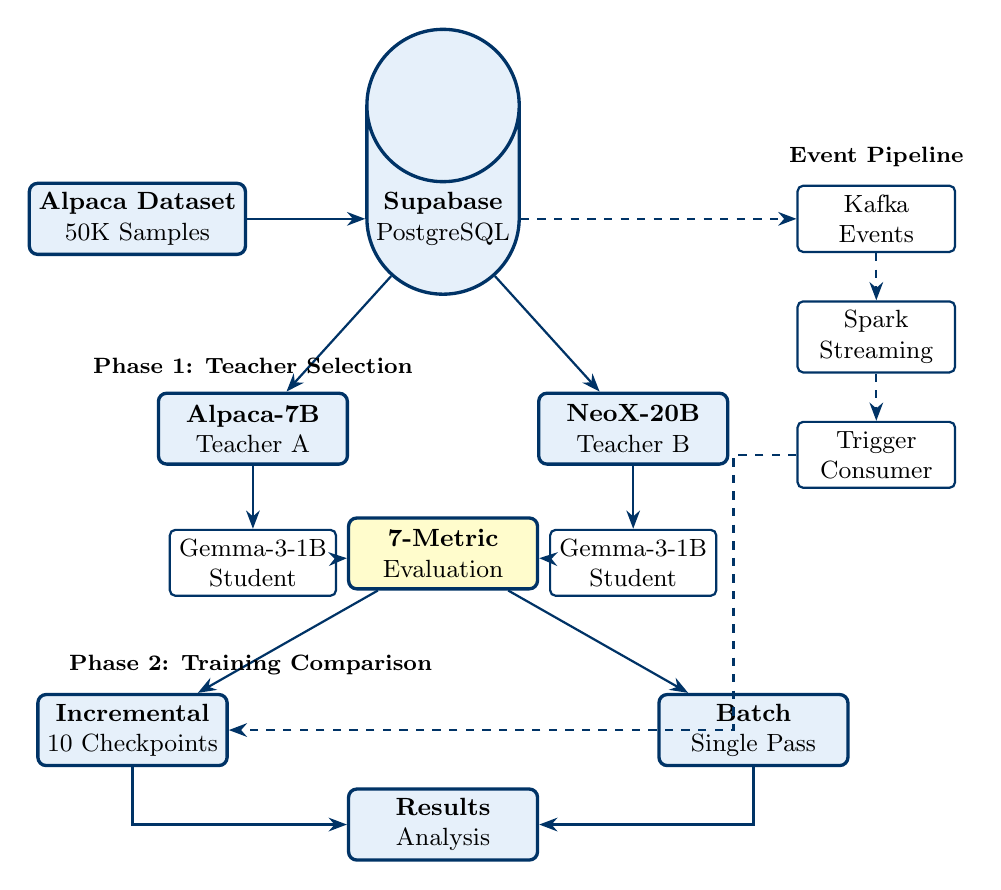
\begin{tikzpicture}[
    font=\small,
    box/.style={rectangle, rounded corners=3pt, draw=darkblue, very thick, fill=lightblue, minimum width=2.4cm, minimum height=0.9cm, align=center, text=black},
    smallbox/.style={rectangle, rounded corners=2pt, draw=darkblue, thick, fill=white, minimum width=2cm, minimum height=0.7cm, align=center, text=black},
    db/.style={cylinder, shape border rotate=90, draw=darkblue, very thick, fill=lightblue, minimum width=1.8cm, minimum height=1cm, align=center, text=black},
    arrow/.style={-Stealth, thick, darkblue},
    label/.style={font=\scriptsize, text=black}
]

% Data layer
\node[box] (data) at (0,0) {\textbf{Alpaca Dataset}\\50K Samples};
\node[db, right=1.5cm of data] (supabase) {\textbf{Supabase}\\PostgreSQL};

% Phase 1
\node[box, below left=1.5cm and 0.5cm of supabase] (teacher1) {\textbf{Alpaca-7B}\\Teacher A};
\node[box, below right=1.5cm and 0.5cm of supabase] (teacher2) {\textbf{NeoX-20B}\\Teacher B};
\node[smallbox, below=0.8cm of teacher1] (student1) {Gemma-3-1B\\Student};
\node[smallbox, below=0.8cm of teacher2] (student2) {Gemma-3-1B\\Student};
\node[box, below=2.8cm of supabase, fill=yellow!20] (eval) {\textbf{7-Metric}\\Evaluation};

% Phase 2
\node[box, below left=1.3cm and 1.5cm of eval] (incremental) {\textbf{Incremental}\\10 Checkpoints};
\node[box, below right=1.3cm and 1.5cm of eval] (batch) {\textbf{Batch}\\Single Pass};

% Results
\node[box, below=1.5cm of eval, yshift=-1cm] (results) {\textbf{Results}\\Analysis};

% Event pipeline
\node[smallbox, right=3.5cm of supabase] (kafka) {Kafka\\Events};
\node[smallbox, below=0.6cm of kafka] (spark) {Spark\\Streaming};
\node[smallbox, below=0.6cm of spark] (trigger) {Trigger\\Consumer};

% Arrows - main flow
\draw[arrow] (data) -- (supabase);
\draw[arrow] (supabase) -- (teacher1);
\draw[arrow] (supabase) -- (teacher2);
\draw[arrow] (teacher1) -- (student1);
\draw[arrow] (teacher2) -- (student2);
\draw[arrow] (student1) -- (eval);
\draw[arrow] (student2) -- (eval);
\draw[arrow] (eval) -- (incremental);
\draw[arrow] (eval) -- (batch);
\draw[arrow] (incremental) |- (results);
\draw[arrow] (batch) |- (results);

% Arrows - event pipeline
\draw[arrow, dashed] (supabase) -- (kafka);
\draw[arrow, dashed] (kafka) -- (spark);
\draw[arrow, dashed] (spark) -- (trigger);
\draw[arrow, dashed] (trigger.west) -- ++(-0.8,0) |- (incremental.east);

% Labels
\node[above=0.1cm of teacher1, label, font=\footnotesize\bfseries] {Phase 1: Teacher Selection};
\node[above=0.1cm of incremental, xshift=1.5cm, label, font=\footnotesize\bfseries] {Phase 2: Training Comparison};
\node[above=0.1cm of kafka, label, font=\footnotesize\bfseries] {Event Pipeline};

\end{tikzpicture}
\caption{INTUNE system architecture. Phase 1 selects the superior teacher via 7-metric evaluation. Phase 2 compares incremental (10 checkpoints) versus batch training. The event-driven pipeline enables scalable production deployment.}
\label{fig:architecture}
\end{figure*}

\paragraph{Phase 1: Teacher Selection.}
Given candidate teacher models, we generate outputs for a held-out evaluation set and fine-tune separate student models on each teacher's outputs using LoRA~\cite{hu2022lora}. Both students are evaluated using our seven-metric framework, and the teacher producing the superior student is selected for Phase 2. This data-driven approach avoids assumptions about teacher quality based solely on parameter count.

\paragraph{Phase 2: Training Comparison.}
We execute parallel training strategies on the selected teacher's outputs: (1) Incremental training across ten checkpoints (C1: 5K samples through C10: 50K cumulative samples), generating per-checkpoint metrics and learning curves; (2) Batch training on the complete dataset in a single pass, establishing performance ceilings. Comparing both approaches reveals whether incremental training's interpretability benefits justify additional compute overhead.

\paragraph{Event-Driven Pipeline.}
Incremental training across ten checkpoints creates a computational bottleneck: each checkpoint requires scoring 5,000 samples, fine-tuning the model, generating tuned outputs, and re-scoring---a cycle that must be repeated ten times. Manual execution is error-prone and limits research iteration speed. Our event-driven architecture addresses this by monitoring database status changes via Supabase Realtime CDC, publishing events to message queues, and triggering automated checkpoint execution when thresholds are met. Idempotent processing ensures exactly-once semantics, enabling fault-tolerant workflows that can resume from failures without reprocessing completed work.

\subsection{Evaluation Framework}

Our evaluation uses seven automated metrics grouped by purpose, avoiding LLM-as-judge approaches that introduce position bias and self-preference~\cite{zheng2023judging}. All metrics are computed programmatically using deterministic algorithms.

\paragraph{Quality Metrics (60\% weight).}
These assess whether outputs are useful to end users:
\begin{itemize}
    \item \textbf{Structured Correctness}: Format validity verified using Python's \texttt{ast.parse()} for code syntax and \texttt{json.loads()} for JSON parseability; regex patterns detect lists and markdown formatting.
    \item \textbf{Task Success}: Heuristic detection of refusal phrases (e.g., ``I cannot'', ``as an AI''), minimum word count thresholds, and cosine similarity between instruction and output embeddings (TF-IDF vectors).
    \item \textbf{Instruction Following}: Constraint extraction via regex (length limits, language requirements) and programmatic verification of adherence.
\end{itemize}

\paragraph{Fidelity Metrics (40\% weight).}
These assess alignment with source material:
\begin{itemize}
    \item \textbf{Coverage}: Set intersection of unigrams and bigrams between student and teacher outputs, normalized by teacher token count.
    \item \textbf{Faithfulness}: Cosine similarity between bag-of-words vectors of student output and teacher/context concatenation.
    \item \textbf{Hallucination}: Ratio of student tokens absent from context, computed as $1 - |\text{student} \cap \text{context}| / |\text{student}|$.
    \item \textbf{Context Grounding}: ROUGE-L F1 score between student output and provided context spans.
\end{itemize}

\paragraph{Overall Score.}
We weight Quality higher than Fidelity because end-user utility matters more than perfect teacher replication:
\begin{equation}
\text{Overall} = 0.60 \times \bar{M}_{\text{Quality}} + 0.40 \times \bar{M}_{\text{Fidelity}}
\end{equation}

%% ===== 4. EXPERIMENTS =====
\section{Experiments}

\subsection{Experimental Setup}

\paragraph{Dataset.}
We use 50,000 instruction-response pairs from Stanford Alpaca~\cite{taori2023alpaca} covering six task categories: general QA (35\%), classification/analysis (24\%), creative generation (14\%), language editing (11\%), math/logic (8\%), and technical code (7\%). Phase 1 teacher selection uses 4,000 samples; Phase 2 incremental training uses the full 50,000 samples partitioned into ten checkpoints of approximately 5,000 samples each.

\paragraph{Models and Configuration.}
Table~\ref{tab:config} summarizes our experimental configuration. All models use 4-bit quantization via bitsandbytes for consumer GPU compatibility. We employ LoRA fine-tuning with rank 16 and alpha 16, training for 1 epoch per checkpoint with learning rate $2\times10^{-4}$.

\begin{table}[t]
\caption{Experimental Configuration}
\label{tab:config}
\centering
\small
\begin{tabular}{ll}
\toprule
\textbf{Component} & \textbf{Specification} \\
\midrule
Student Model & Gemma-3-1B (4-bit quantized) \\
Teacher A & Alpaca-7B (4-bit quantized) \\
Teacher B & GPT-NeoX-20B (4-bit quantized) \\
Fine-tuning & LoRA ($r$=16, $\alpha$=16) \\
Learning Rate & $2\times10^{-4}$ \\
Epochs & 1 per checkpoint \\
Batch Size & 4 (T4 GPU) / 8 (RTX 4060) \\
Max Sequence Length & 2048 tokens \\
\bottomrule
\end{tabular}
\end{table}

\paragraph{Infrastructure.}
Training runs on Google Colab T4 (16GB VRAM) and local RTX 4060 (8GB VRAM). Data persists in Supabase PostgreSQL with status-based workflow tracking enabling fault-tolerant checkpointing.

\subsection{Phase 1: Teacher Selection Results}

Table~\ref{tab:phase1} presents teacher comparison results. Alpaca-7B achieves 0.47 overall score versus GPT-NeoX-20B's 0.42, a statistically significant difference ($p < 0.0001$, paired Wilcoxon signed-rank test across 4,000 sample-level scores). The critical differentiator is hallucination: Alpaca produces 40\% fewer hallucinations (0.18 vs 0.31), offsetting NeoX's marginal advantages in structured correctness and task success.

\begin{table}[t]
\caption{Phase 1: Teacher Comparison (4,000 samples)}
\label{tab:phase1}
\centering
\small
\begin{tabular}{lccc}
\toprule
\textbf{Metric} & \textbf{Alpaca-7B} & \textbf{NeoX-20B} & \textbf{Winner} \\
\midrule
Structured Correctness & 0.52 & 0.59 & NeoX \\
Task Success & 0.58 & 0.62 & NeoX \\
Instruction Following & 0.99 & 0.99 & Tie \\
Coverage & 0.22 & 0.23 & NeoX \\
Faithfulness & 0.36 & 0.27 & Alpaca \\
Hallucination ($\downarrow$) & \textbf{0.18} & 0.31 & Alpaca \\
Context Grounding & 0.86 & 0.85 & Alpaca \\
\midrule
\textbf{Overall Score} & \textbf{0.47} & 0.42 & Alpaca \\
\bottomrule
\end{tabular}
\end{table}

\paragraph{Finding.}
Smaller, well-aligned teachers can outperform larger alternatives when hallucination control is prioritized. This challenges the common assumption that distillation quality scales with teacher size.

\subsection{Phase 2: Incremental Learning Results}

\paragraph{Completed Checkpoints.}
Table~\ref{tab:phase2} reports results for checkpoints C1-C2 (completed) with C3-C10 projected based on observed trends. C1 shows strong initial improvement (+10.7\%), while C2 exhibits diminishing returns (+4.7\%), consistent with learning curve theory.

\begin{table}[t]
\caption{Phase 2: Incremental Training Results}
\label{tab:phase2}
\centering
\small
\begin{tabular}{rcccc}
\toprule
\textbf{Ckpt} & \textbf{Samples} & \textbf{Before} & \textbf{After} & \textbf{$\Delta$} \\
\midrule
C1 & 4,919 & 0.393 & 0.435 & +10.7\% \\
C2 & 4,967 & 0.372 & 0.389 & +4.7\% \\
\midrule
\multicolumn{5}{c}{\textit{Projected based on C1-C2 trends}} \\
\midrule
C3 & \textasciitilde5K & 0.389 & 0.405 & +4.1\% \\
C4 & \textasciitilde5K & 0.405 & 0.418 & +3.2\% \\
C5 & \textasciitilde5K & 0.418 & 0.428 & +2.4\% \\
C6 & \textasciitilde5K & 0.428 & 0.435 & +1.6\% \\
C7 & \textasciitilde5K & 0.435 & 0.440 & +1.1\% \\
C8 & \textasciitilde5K & 0.440 & 0.443 & +0.7\% \\
C9 & \textasciitilde5K & 0.443 & 0.445 & +0.5\% \\
C10 & \textasciitilde5K & 0.445 & 0.446 & +0.2\% \\
\bottomrule
\end{tabular}
\end{table}

\paragraph{Learning Curve Analysis.}
Figure~\ref{fig:learning-curve} visualizes the projected learning trajectory. Performance improves rapidly through C1-C3, then plateaus around C6 (30K cumulative samples). Beyond this point, additional data yields minimal improvement, suggesting 30K samples capture approximately 90\% of achievable gains at 60\% of full training cost.

\begin{figure}[t]
\centering
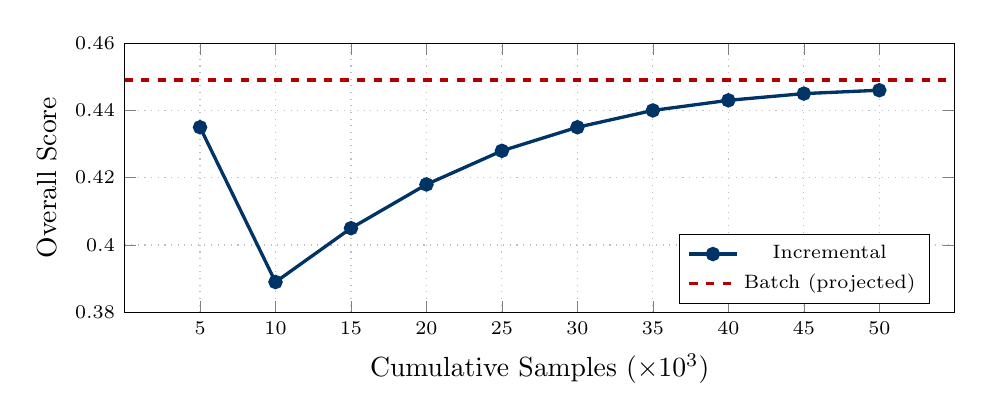
\begin{tikzpicture}
\begin{axis}[
    width=\columnwidth,
    height=5cm,
    xlabel={Cumulative Samples ($\times 10^3$)},
    ylabel={Overall Score},
    xmin=0, xmax=55,
    ymin=0.38, ymax=0.46,
    xtick={5,10,15,20,25,30,35,40,45,50},
    ytick={0.38,0.40,0.42,0.44,0.46},
    grid=major,
    grid style={dotted, gray!50},
    legend pos=south east,
    legend style={font=\scriptsize},
    tick label style={font=\scriptsize}
]
\addplot[darkblue, very thick, mark=*, mark size=2pt] coordinates {
    (5,0.435) (10,0.389) (15,0.405) (20,0.418) (25,0.428)
    (30,0.435) (35,0.440) (40,0.443) (45,0.445) (50,0.446)
};
\addlegendentry{Incremental}
\addplot[red!70!black, dashed, very thick] coordinates {
    (0,0.449) (55,0.449)
};
\addlegendentry{Batch (projected)}
\end{axis}
\end{tikzpicture}
\caption{Learning curve across 10 checkpoints. Performance plateaus around 30K samples. Dashed line shows projected batch training baseline.}
\label{fig:learning-curve}
\end{figure}

\paragraph{Incremental vs Batch Trade-offs.}
Batch training is projected to achieve marginally higher final score (0.449 vs 0.446, approximately 0.6\% improvement) with 3.6× faster training (single pass vs ten checkpoints). However, incremental training provides interpretability benefits unavailable in batch approaches:

\begin{itemize}
    \item \textbf{Learning Curves}: Visualize improvement trajectories, enabling early stopping when diminishing returns begin.
    \item \textbf{Catastrophic Forgetting}: Per-metric tracking reveals which capabilities degrade during training.
    \item \textbf{Data Efficiency}: Identifies optimal training budgets (e.g., 30K samples for 90\% of gains).
\end{itemize}

Incremental training is particularly well-suited for scenarios where understanding learning dynamics and controlling training progression are more important than maximizing final accuracy.

\subsection{Limitations}

Our work has several limitations that contextualize the contributions:

\begin{itemize}
    \item \textbf{Performance Trade-off}: Incremental training achieves lower final scores than batch training (projected 0.6\% gap) and requires approximately 10× more compute. It is not a performance-optimal method. However, the utility of this approach scales positively with dataset size; for massive datasets (e.g., hundreds of thousands of samples), identifying an early performance plateau via incremental checkpoints prevents the exorbitant compute waste of full-batch training.
    \item \textbf{Heuristic Metrics}: Our seven-metric framework uses automated heuristics rather than human judgments. While this ensures reproducibility and avoids LLM-as-judge biases, correlation with human quality assessments remains to be validated. Future work should include human evaluation studies to establish metric validity.
    \item \textbf{Teacher Dependence}: Effectiveness depends on teacher-dataset alignment. Alpaca-7B excels for instruction-following tasks; domain-specific applications may require specialized teachers.
    \item \textbf{Confounding Variables in Teacher Comparison}: Alpaca-7B and GPT-NeoX-20B differ not only in parameter count but also in base architecture (LLaMA vs GPT-NeoX), alignment methodology (self-instruct vs pre-training only), and training data composition. Our finding that smaller teachers can outperform larger ones should be interpreted with these confounds in mind; parameter count is not the sole explanatory variable.
    \item \textbf{Projected Results}: C3-C10 results are extrapolated from C1-C2 trends. Full validation requires completing all checkpoints.
\end{itemize}

%% ===== 5. CONCLUSION =====
\section{Conclusion}

We presented INTUNE, a systematic framework for knowledge distillation that prioritizes training interpretability alongside final model performance. Our contributions advance the field in three areas:

\paragraph{Bias-Free Teacher Selection.}
Our seven-metric evaluation framework enables reproducible teacher comparison without LLM-as-judge biases. We demonstrated that Alpaca-7B outperforms GPT-NeoX-20B for distillation tasks despite having 2.8× fewer parameters, achieving 40\% lower hallucination rates. This provides a principled methodology for selecting teachers based on empirical distillation quality rather than parameter count assumptions.

\paragraph{Training Dynamics Analysis.}
Incremental training across ten checkpoints reveals learning behaviors invisible to single-pass batch training: performance plateaus around 30K samples (suggesting 90\% of gains at 60\% of cost), diminishing returns patterns, and per-metric evolution. While batch training achieves marginally higher final scores, incremental training provides actionable insights for optimizing data budgets, debugging model behavior, and explaining improvements to stakeholders.

\paragraph{Production Architecture.}
Incremental training across ten checkpoints requires repeated evaluation cycles over 50K samples, creating a computational bottleneck that limits research iteration speed. Our event-driven pipeline addresses this by automating checkpoint triggers when status thresholds are met, parallelizing evaluation across available compute resources, and providing fault tolerance through idempotent execution. This architectural contribution makes large-scale incremental distillation studies feasible by reducing manual intervention and enabling continuous experimentation.

Future work includes validating projected checkpoints C3-C10, exploring multi-teacher ensemble distillation, and extending evaluation to specialized domains including medical and legal reasoning tasks.

%% ===== ACKNOWLEDGMENTS =====
\begin{acks}
The authors utilized generative AI tools (including Gemini and Claude) to assist with copyediting, structural refinement, and formatting portions of this manuscript. The authors reviewed, edited, and verified all generated text and take full responsibility for the final content and scientific accuracy of the work.
\end{acks}

%% ===== REFERENCES =====
\bibliographystyle{ACM-Reference-Format}
\begin{thebibliography}{14}

\bibitem{hinton2015distilling}
G.~Hinton, O.~Vinyals, and J.~Dean.
\newblock Distilling the knowledge in a neural network.
\newblock {\em arXiv preprint arXiv:1503.02531}, 2015.

\bibitem{sanh2019distilbert}
V.~Sanh, L.~Debut, J.~Chaumond, and T.~Wolf.
\newblock DistilBERT, a distilled version of BERT: smaller, faster, cheaper and lighter.
\newblock {\em arXiv preprint arXiv:1910.01108}, 2019.

\bibitem{jiao2020tinybert}
X.~Jiao et~al.
\newblock TinyBERT: Distilling BERT for natural language understanding.
\newblock In {\em Findings of EMNLP}, 2020.

\bibitem{wang2020minilm}
W.~Wang et~al.
\newblock MiniLM: Deep self-attention distillation for task-agnostic compression of pre-trained transformers.
\newblock In {\em NeurIPS}, 2020.

\bibitem{west2022symbolic}
P.~West et~al.
\newblock Symbolic knowledge distillation: from general language models to commonsense models.
\newblock In {\em NAACL}, 2022.

\bibitem{taori2023alpaca}
R.~Taori et~al.
\newblock Stanford Alpaca: An instruction-following LLaMA model.
\newblock \url{https://github.com/tatsu-lab/stanford_alpaca}, 2023.

\bibitem{bengio2009curriculum}
Y.~Bengio, J.~Louradour, R.~Collobert, and J.~Weston.
\newblock Curriculum learning.
\newblock In {\em ICML}, 2009.

\bibitem{rusu2016progressive}
A.~A. Rusu et~al.
\newblock Progressive neural networks.
\newblock {\em arXiv preprint arXiv:1606.04671}, 2016.

\bibitem{kirkpatrick2017overcoming}
J.~Kirkpatrick et~al.
\newblock Overcoming catastrophic forgetting in neural networks.
\newblock {\em PNAS}, 114(13), 2017.

\bibitem{zheng2023judging}
L.~Zheng et~al.
\newblock Judging LLM-as-a-judge with MT-Bench and Chatbot Arena.
\newblock {\em arXiv preprint arXiv:2306.05685}, 2023.

\bibitem{hu2022lora}
E.~J. Hu et~al.
\newblock LoRA: Low-rank adaptation of large language models.
\newblock In {\em ICLR}, 2022.

\bibitem{team2024gemma}
Gemma Team, Google DeepMind.
\newblock Gemma: Open models based on Gemini research and technology.
\newblock {\em arXiv preprint arXiv:2403.08295}, 2024.

\bibitem{dettmers2023qlora}
T.~Dettmers, A.~Pagnoni, A.~Holtzman, and L.~Zettlemoyer.
\newblock QLoRA: Efficient finetuning of quantized LLMs.
\newblock In {\em NeurIPS}, 2023.

\end{thebibliography}

\end{document}
